\section{VIEW Set Graphical View}

\subsection{Usage}

The \verb|view| function sets the view into the current plot.
The simplest form is
\begin{verbatim}
  view(n)
\end{verbatim}
where \verb|n=2| sets a standard view (azimuth 0 and elevation 90),
and \verb|n=3| sets a standard 3D view (azimuth 37.5 and elevation 30).
With two arguments,
\begin{verbatim}
  view(az,el)
\end{verbatim}
you set the viewpoint to azimuth \verb|az| and elevation \verb|el|.
\subsection{Example}

Here is a 3D surface plot shown with a number of viewpoints.
First, the default view for a 3D plot.
\begin{verbatim}
--> x = repmat(linspace(-1,1),[100,1]);
--> y = x';
--> r = x.^2+y.^2;
--> z = exp(-r*3).*cos(5*pi*r);
--> surf(x,y,z);
--> axis equal
--> view(3)
\end{verbatim}


\centerline{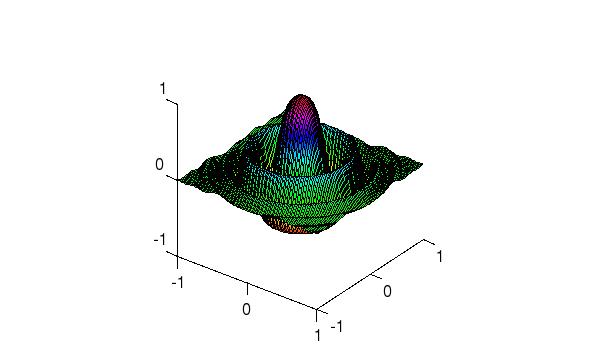
\includegraphics[width=8cm]{view1}}

Next, we look at it as a 2D plot
\begin{verbatim}
--> surf(x,y,z);
--> axis equal
--> view(2)
\end{verbatim}


\centerline{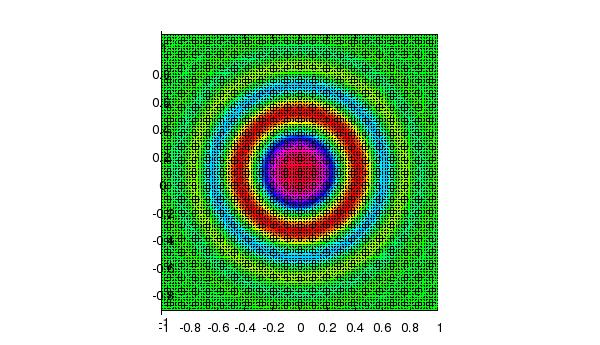
\includegraphics[width=8cm]{view2}}

Finally, we generate a different view of the same surface.
\begin{verbatim}
--> surf(x,y,z);
--> axis equal
--> view(25,50);
\end{verbatim}


\centerline{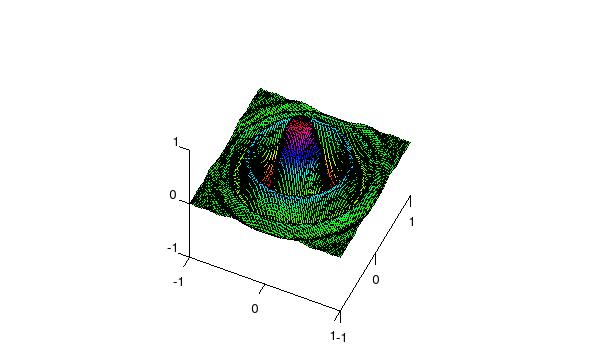
\includegraphics[width=8cm]{view3}}

